\chapter{Model Application}
\label{chp:chapter4}
\graphicspath{{figures/}{figures/chapter4/}}

\section{Overview}
In this chapter, we apply the Resiliency Model to evaluate the effects of link
loss or degradation on the USTM network. We do this by applying the model to scenarios
where critical highway links have been removed from the USTM network. This
chapter includes first, a detailed analysis of a single scenario, where I-80
between Salt Lake and Tooele Counties is severed. We then compare the model
output to an alternative method that measures only the change in travel
time and does not allow for mode or destination choice. The model was then
applied to 41 individual scenarios, with 40 of those scenarios involving link
closure scenarios throughout the state.

\section{Vulnerable Link Identification}
Two methodologies were developed to identify vulnerable network links in
Utah. The first method resembles the process used by AEM to determine
threat categories and threat proximity thresholds to highway links. The
second method uses an online Risk Priority Analysis map created by UDOT to identify points of interest based on exisiting risk analysis data. Additional
points of interest were identified by the research team or by UDOT officials, who have a familiar working knowledge of the USTM network. Using this second
method, links were identified due to their location in relation to
population centers, remote geographic location, proximitiy to other highway facilities, were known to be at risk due to geologic or geographic features, or
because they were suspected choke points in the network.

After identifying locations of interest, we now apply the model to compare the results of 40 scenarios. In each scenario, an individual highway
facility is removed from the model highway network. Each of these scenario locations is shown in Figure \ref{fig:linksmap}, and is identified in a report by
\cite{aem2017} or the research team using the methodology described. A detailed analysis of the results of a single scenario will be done, followed by a
more general analysis for all 40 scenarios considered in the Resiliency Model.

\section{Localized Scenario Analysis}

This section outlines an in-depth, localized analysis that was conducted to ensure
the Resiliency Model was accurately describing trips with OD pairs in the
targeted area around a severed link. This analysis was done on a link between
Tooele and Salt Lake City, Utah. This detailed analysis is useful because it
provides a closer look at the way the Resiliency Model works, capturing trips
between two population centers.

Scenario 50, which is located along I-80 between Tooele and Salt Lake Counties
was examined here. The localized analysis shows that the majority of trips
affected by damage to this link either originate or terminate in one of the
two counties, as expected. These results can be seen in Table
\ref{tab:tooeletable}. Another method we used to compare results against is
the travel time method,
which serves to capture trips that have fixed OD pairs such as freight and
recreational trips. This localized analysis also looks at this method.

Table \ref{tab:tooeletable} compares trips and the overall costs between the
logsum and travel time methods, the specific cost for trips originating in
Tooele County and ending in Salt Lake County. We can see that the logsum
method captures about
\$54,000 of expenses experienced by road users due to the closure of the
link. Specifically, between Tooele and Salt Lake Counties, the logsum based analysis using the Resiliency
Model captures \$21,000 of
expense, which is approximately 38\% of the total expense experienced
statewide. A further breakdown of expenses experienced at the local level
between Tooele and Salt Lake Counties
can be seen Table \ref{tab:tooeletable2}.

The data supports the conclusion that the Resiliency Model is effectively
capturing trips between Tooele and Salt Lake Counties based on the percent capture
rates in Table \ref{tab:tooeletable2}. Additionally, when we look at the
travel time method of analysis, we can see that the costs at both the local and
statewide levels are much greater with about \$437,000 and \$407,000
respectively estimated as the costs due to just the increase in travel time, not using
the logit-based model.

\begin{table}
\caption{\label{tab:tooeletable}Localized Analysis Results}

\centering
%\begin{adjustbox}{width=0.9\textwidth}
\begin{tabular}[t]{lrrrrrr}
\toprule
Trip Purpose & \multicolumn{2}{c}{ \makecell{Whole Network Cost\\ (Dollars per Day)}} & \multicolumn{2}{c}{\makecell{Tooele - SLC Cost \\(Dollars per Day)}} & \multicolumn{2}{c}{Base Trips}\\
\midrule
 & \makecell{Logsum\\ Method} & \makecell{Travel Time\\ Method} & \makecell{Logsum \\Method} & \makecell{Travel Time\\ Method} & \makecell{ Tooele - \\ SLC } &
\makecell{Whole\\Network} \\
\midrule
HBW & \$15397.06 & \$244275.72 & \$12143.11 & \$233373.56 & 7980 & 1684141\\
HBO & \$12882.89 & \$108412.94 & \$3577.62 & \$98163.53 & 6665.86 & 4593248\\
NHB & \$25635.92 & \$84712.36 & \$5025.24 & \$75361.98 & 1025
& 2611185\\
\midrule
\addlinespace
REC & \$398.72 & \$398.72 & \$40.73 & \$40.73 & 3 & 2385\\
XXP & \$3690.26 & \$55870.17 & \$55870.17 & \- & 0 & 22350\\
Freight & \$911254.89 & \$10883835.01 & \$111772.5 & \$111772.5 & 515811 &
875183\\
Total Logsum & \$53897.87 & \$437401.02 & \$20745.97 & \$406899.06 &
15672 & 8888574\\
Total & \$969241.74 & \$437401.02 & \$132559.20 & \$406899.06 & 531486 & 9788493\\
\bottomrule
\end{tabular}
%\end{adjustbox}
\end{table}

\begin{table}

\caption{\label{tab:tooeletable2}Localized Analysis Cost Capture Rates}
\centering
\begin{tabular}[t]{ccc}
\toprule
 & Logsum & Travel Time\\
\midrule
HBW & 0.7896 & 0.9554 \\
HBO & 0.2777 & 0.9055 \\
NHB & 0.1960 & 0.8896 \\
\bottomrule
\end{tabular}
\end{table}

The logsum and travel time methods can be broken down into the overall costs and the
comparable costs. The comparable costs are made up of those purposes which are
included in both the Resiliency Model and in the travel time method for determining
cost. HBW, HBO, and NHB trip purposes can be compared because all three trip purposes
are represented by each method of cost estimation.

The travel time method measures the difference in travel time between the base scenario and any other scenario caused by link closure, and then multiplies that
difference by the VOT for each trip purpose and the number of trips estimated for
each trip purpose. For external trips, freight trips, and REC trips, these were all
extracted directly from USTM. Attempting to include a calculation of the costs
associated with increased travel time for freight trips, external trips, and REC
trips allows a better estimation of the true cost experienced by all road users, not
just those who are included in the Resiliency Model.

The HBW, HBO, and NHB purposes are estimated using the logsum portion of the
Resiliency Model. Calculating the costs associated with the change in logsum
provides estimations of the costs experienced by road users due to link loss
that account for user choice of mode and destination. The logit-based model
employed in the Resiliency Model ultimately provides lower estimates of the
total disbenefit, and therefore cost, experienced by road users due to link
degradation or loss for the purposes included for analysis. However, the
logsum calculation is only used for three purposes in the USTM model. A way to
account for freight trips, REC trips, and trips that occur between external
nodes must also be found. These trip purposes typically have fixed origins
nd destinations. As such, a way to account for all purposes must be developed.
Thus, by combining elements from the travel time method and the Resiliency Model, an estimate can be made that represents all traffic on the USTM network.

\begin{figure}

{\centering 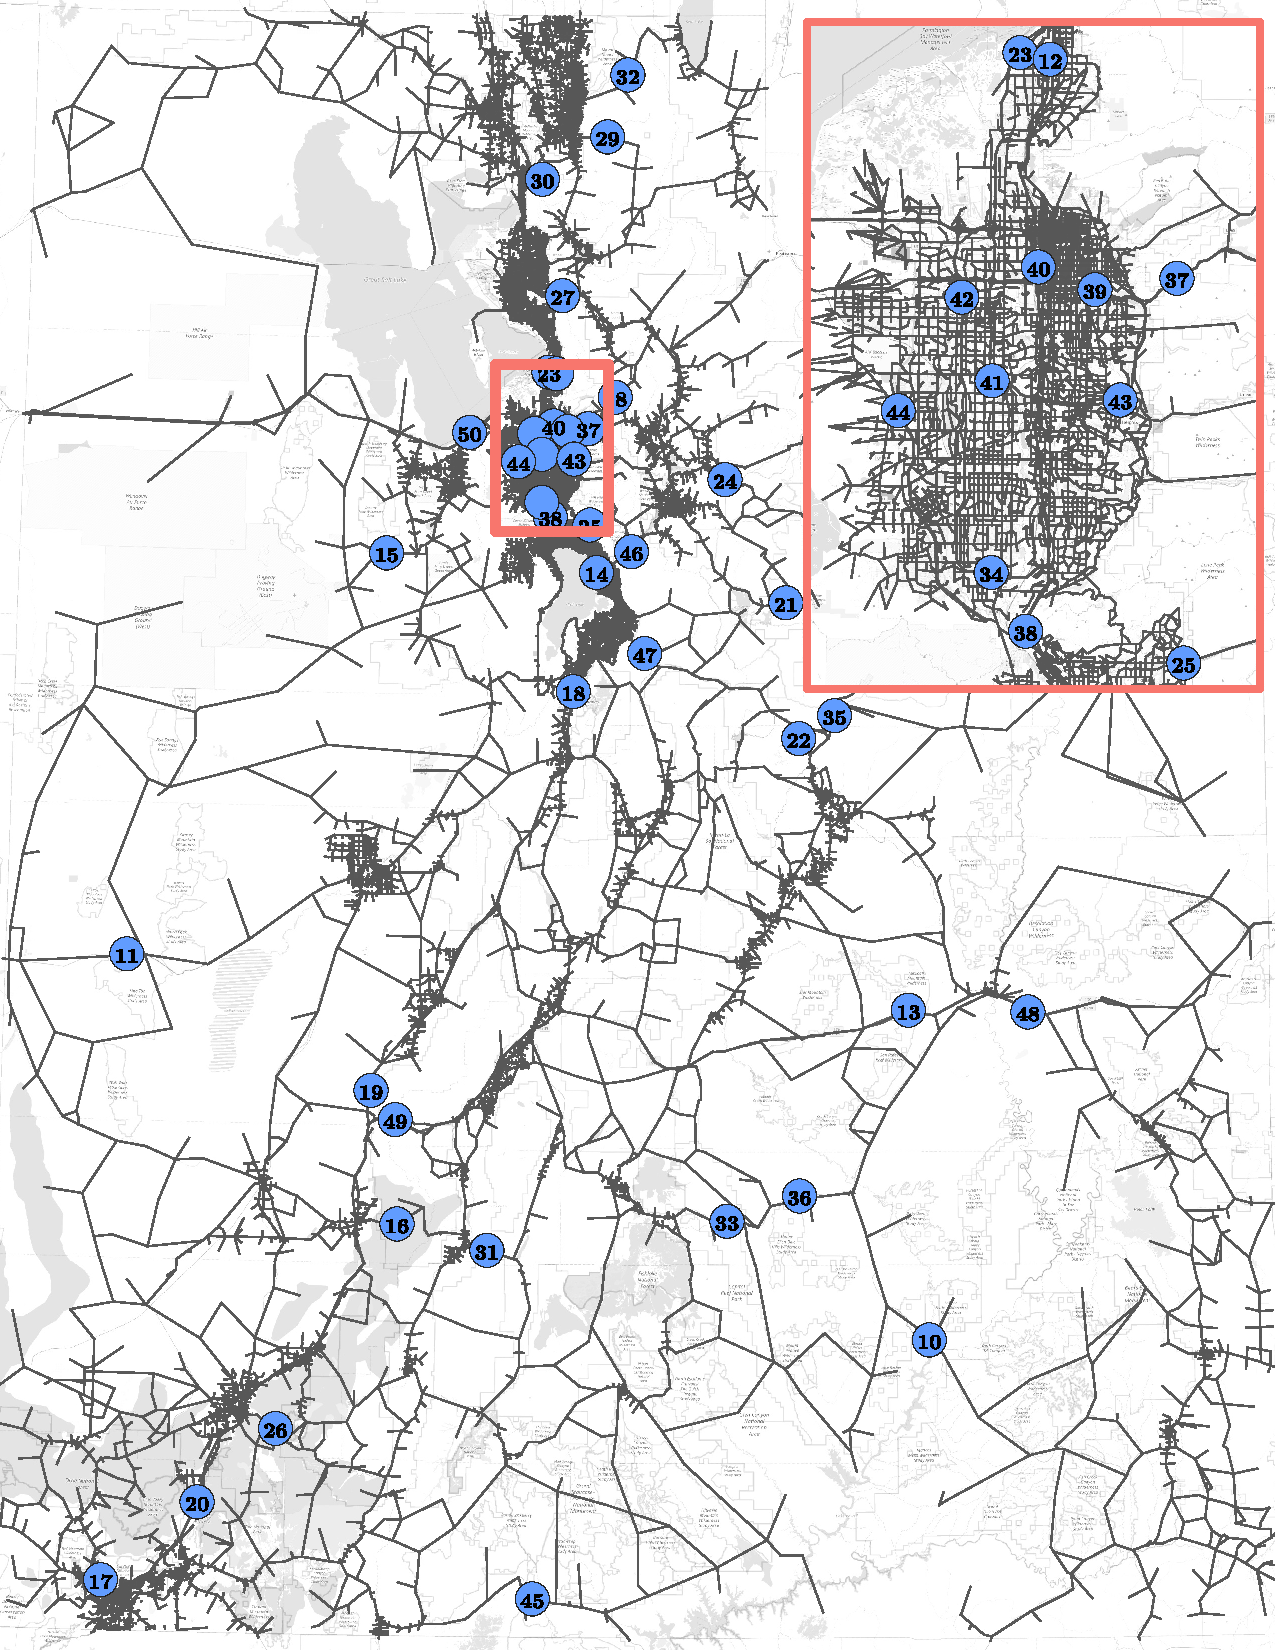
\includegraphics[width=0.95\linewidth]{figures/chapter4/resiliency_links_map.pdf}}

\caption{Links Identified for Analysis.}
\label{fig:linksmap}
\end{figure}

The following sections will present the results of the 40 scenarios analyzed.
First, Table \ref{tab:linkresults} shows each of the scenarios we examined,
labeled simply as ``10'' for scenario 10, and ``11'' for scenario 11, along with the
change in accessibility, $\Delta$ Logsum, and the Cost Value in dollars per day
associated with link closure. Other identifying information, such as route
numbers or street names and geographic or other identifying descriptions about
the locations where the link was cut, are also provided.

The logsum method results are as follows in Table \ref{tab:linkresults}.
The results are ranked from the road with the largest (most positive
cost) to the road with the smallest cost. We can see that scenario 27, which
corresponds to I-84 between Ogden and Morgan, experiences the largest cost
per day according to the Resiliency Model. Following scenario 27, scenarios 50, 37, 30,
and 17 make up the five most important roads according to the cost estimation
provided by the Resiliency Model. Each of the roads in these scenarios --- with the exception
of SR-18 in St. George --- is an interstate or state highway facility in
northern Utah, which is heavily populated. Some scenarios, such as scenario 10,
scenario 11, or scenario 33, are roads that are located in remote parts of the state, and
experience no measurable change to HBW, HBO, or NHB traffic. This is
likely due to the remoteness of the geographic location of the highway
link that was cut. A ranking is provided for all of the examined scenarios in Table \ref{tab:linkresults}.

\begin{table}


\caption{\label{tab:linkresults}Logsum Analysis Results}
\centering
\begin{tabular}[t]{crrll}
\toprule
Scenario & $\Delta$ Logsum & \makecell{Cost \\(Dollars per Day)} & Route & Location\\
\midrule
27 & -23830.208 & 14893880.00 & I-84 & between Ogden and Morgan\\
50 & -19686.788 & 12304242.50 & I-80 & between SLC and Tooele\\
37 & -8932.691 & 5582931.88 & I-80 & in Parley's Canyon\\
30 & -7511.948 & 4694967.50 & US-91 & between Brigham City \& Mantua\\
17 & -5243.828 & 3277392.50 & SR-18 & just North of St. George\\
46 & -4911.457 & 3069660.63 & SR-189 & up Provo Canyon near Vivian Park\\
38 & -4422.194 & 2763871.25 & I-15 & at the Point of the Mount\\
18 & -3186.967 & 1991854.38 & I-15 & in Rocky Ridge (between Payson \& Nephi)\\
42 & -2657.614 & 1661008.75 & Bangerter & near West Valley City\\
41 & -1700.167 & 1062604.38 & I-215 & near Taylorsville\\
25 & -1139.020 & 711887.50 & Timp Hwy & at the mouth of AF Canyon\\
24 & -387.467 & 242166.88 & UT-35 & outside of Francis\\
23 & -297.882 & 186176.25 & Legacy & near West Bountiful\\
20 & -253.712 & 158570.00 & I-15 & near New Harmony\\
47 & -142.671 & 89169.38 & US-6 & Spanish Fork Canyon at Diamond Fork Rd\\
26 & -125.740 & 78587.50 & SR-14 & in Cedar Canyon\\
15 & -67.634 & 42271.25 & SR-199 & near Rush Valley\\
32 & -60.883 & 38051.88 & US-89 & between Logan and Bear Lake\\
14 & -45.386 & 28366.25 & I-15 & in Orem between Univ. Ave \& Center St\\
29 & -41.595 & 25996.88 & SR-101 & East of Hyrum\\
31 & -40.108 & 25067.50 & SR-62 & East of Kingston\\
22 & -30.394 & 18996.25 & US-6 & in Carbon County North of Helper\\
49 & -17.768 & 11105.00 & I-70 & near Richfield \& Fillmore\\
45 & -17.029 & 10643.13 & US-89 & near Arizona Border\\
21 & -11.267 & 7041.88 & US-40 & East of Strawberry Reservoir\\
36 & -10.170 & 6356.25 & SR-24 & near Steamboat Point\\
16 & -9.724 & 6077.50 & SR-153 & between Beaver \& Junction\\
48 & -9.717 & 6073.13 & I-70 & near Green River (NW of Moab)\\
19 & -7.623 & 4764.38 & I-15 & near I-70 \& Fillmore\\
35 & -3.762 & 2351.25 & SR-191 & between Helper \& Duchesne\\
13 & -0.135 & 84.38 & I-70 & at Dragon Point (W of Green River)\\
28 & -0.103 & 64.38 & SR-65 & border of Salt Lake \& Morgan Counties\\
10 & 0.000 & 0.00 & SR-95 & near Hite\\
11 & 0.000 & 0.00 & US-6 & near King Top\\
33 & 0.000 & 0.00 & SR-24 & in Capitol Reef National Park\\
12 & 894.999 & -559374.38 & I-15 & in Bountiful\\
44 & 2149.291 & -1343306.88 & UT-85 & West of West Jordan\\
43 & 4043.132 & -2526957.50 & I-215 & near Cottonwood Heights\\
40 & 5576.276 & -3485172.50 & I-15 & in SLC between 2100 S \& 1300 S\\
39 & 7434.744 & -4646715.00 & I-80 & in SLC near Sugar House and 1300 E\\
34 & 9362.283 & -5851426.88 & Bangerter & near Bluffdale\\
\bottomrule
\end{tabular}
\end{table}

Table \ref{tab:timeresults} contains the ranking results from the travel
time method. Here, we see that the first five roads differ from the
results of the logsum model. Scenario, road 48 becomes the most important
road due to costs experienced. Scneario 48 is a part of I-70 near Green River,
Utah. The other four roads that make up the top five most important roads
in the travel time method analysis are scenario 13, scenario 20, scenario 50, and scenario
49. Some of these scenarios appear in both the logsum and travel time method results. This is not unexpected, because each of these facilites is a main arterial in the region where they are located, and are interstate highways carrying large amounts of private passenger vehicles and freight.
Here again, several of the roads that are most important are located in
Northern Utah. It is important to note that the main driving factor as to
why a road was important or not in the travel time analysis was how much
freight and external traffic it experienced along that route. Including
the freight, even with the logsum results, changes the rankings
drastically because of the significantly higher value of time associated
with freight trips.

\begin{table}

\caption{\label{tab:timeresults}Travel Time Analsyis Results ($\Delta$ Cost in Dollars per Day)}
\makebox[\linewidth]{
\centering
\begin{tabular}[t]{lrrrrrrrrrr}
\toprule
ROAD & \makecell{IIF} & \makecell{XXF} & \makecell{IXF} & \makecell{HBW} & \makecell{HBO} & \makecell{NHB} & \makecell{REC} & \makecell{XXP} & \makecell{TIME($\Delta$ hr)} & \makecell{Total Cost}\\
\midrule
48 & 990780 & 84546937 & 0 & 196 & 257 & 29 & 15448 & 417992 & 8629842 & 85971638\\
13 & 83991 & 25130678 & 0 & 0 & 3 & 0 & 211 & 95273 & 1273123 & 25310156\\
20 & 568558 & 18716735 & 175 & 2873 & 2640 & 1209 & 11372 & 234814 & 9060110 & 19538377\\
50 & 608787 & 10274995 & 54 & 244276 & 108413 & 84712 & 399 & 55870 & 2096105 & 11377505\\
49 & 307906 & 7810609 & 0 & 78 & 59 & 18 & 156 & 29827 & 1035612 & 8148653\\
18 & 3935367 & 1847822 & 1148 & 20436 & 21164 & 15363 & 13840 & 143890 & 15621368 & 5999030\\
27 & 185449 & 4359448 & 664 & 35891 & 20811 & 52515 & 208 & 9609 & 637589 & 4664596\\
19 & 2307693 & 1069414 & 104 & 67 & 70 & 13 & 6829 & 94820 & 7376204 & 3479012\\
37 & 1080281 & 978882 & 1128 & 46220 & 36178 & 37632 & 675 & 5669 & 854865 & 2186665\\
47 & 1411715 & 616355 & 8 & 1632 & 373 & 469 & 2600 & 14012 & 4031623 & 2047164\\
38 & 1341423 & 391182 & 153 & 75916 & 88791 & 84970 & 2486 & 17293 & 3582190 & 2002214\\
14 & 712060 & 238361 & 5 & 31899 & 35722 & 38115 & 1724 & 10900 & 2236074 & 1068785\\
30 & 909936 & 804 & 515 & 15379 & 12883 & 25636 & 624 & 3690 & 1917099 & 969467\\
39 & 168147 & 662430 & 298 & 15713 & 15091 & 19513 & 135 & 2821 & 135905 & 884148\\
22 & 421712 & 260885 & 8 & 4 & 28 & 17 & 1164 & 4843 & 1384531 & 688662\\
45 & 864 & 550941 & 146 & 184 & 233 & 79 & 13 & 40330 & 90793 & 592790\\
21 & 537843 & 0 & 0 & 26 & 90 & 39 & 423 & 3398 & 569867 & 541819\\
40 & 266206 & 104007 & 1 & 19183 & 19130 & 20512 & 267 & 3233 & 587396 & 432539\\
12 & 299330 & 78183 & 0 & 12586 & 9575 & 12508 & 251 & 3446 & 638924 & 415879\\
35 & 181287 & 0 & 0 & 17 & 70 & 1 & 355 & 2691 & 1087149 & 184421\\
46 & 80594 & 1041 & 100 & 15112 & 21010 & 12684 & 924 & 172 & 1316491 & 131637\\
41 & 15154 & 0 & 0 & 11092 & 17749 & 22621 & 44 & 0 & 21341 & 66660\\
34 & 19511 & 0 & 0 & 8203 & 11806 & 14453 & 57 & 0 & 51735 & 54031\\
32 & 47715 & 809 & 1 & 736 & 597 & 125 & 5 & 0 & 275279 & 49988\\
43 & 4898 & 0 & 32 & 6215 & 10070 & 13886 & 84 & 0 & 17690 & 35186\\
16 & 30533 & 0 & 0 & 35 & 1 & 31 & 118 & 0 & 6675 & 30719\\
42 & 4320 & 0 & 1 & 6624 & 3956 & 4712 & 1 & 0 & 1983 & 19613\\
17 & 2085 & 0 & 0 & 2384 & 3351 & 6416 & 1 & 0 & 45246 & 14238\\
44 & 3496 & 0 & 0 & 3578 & 1910 & 5214 & 2 & 0 & 4535 & 14200\\
11 & 7577 & 0 & 0 & 0 & 3 & 0 & 1 & 0 & 93374 & 7580\\
24 & 1884 & 0 & 0 & 847 & 276 & 1829 & 1 & 0 & 68330 & 4837\\
33 & 4089 & 0 & 0 & 3 & 5 & 0 & 24 & 0 & 44973 & 4121\\
25 & 56 & 0 & 0 & 516 & 273 & 1852 & 0 & 0 & 1116 & 2698\\
36 & 1920 & 0 & 0 & 13 & 34 & 13 & 18 & 0 & 30447 & 1997\\
26 & 733 & 0 & 0 & 261 & 215 & 189 & 18 & 0 & 16305 & 1417\\
31 & 260 & 0 & 0 & 325 & 483 & 158 & 1 & 0 & 36542 & 1225\\
10 & 346 & 0 & 0 & 0 & 0 & 0 & 780 & 0 & 79258 & 1126\\
15 & 210 & 0 & 0 & 221 & 258 & 67 & 4 & 0 & 19340 & 761\\
23 & 168 & 0 & 0 & 85 & 53 & 124 & 0 & 0 & 226 & 430\\
29 & 2 & 0 & 0 & 122 & 0 & 62 & 0 & 0 & 6222 & 187\\
28 & 6 & 0 & 0 & 0 & 0 & 0 & 13 & 0 & 925 & 19\\
Base & 0 & 0 & 0 & 0 & 0 & 0 & 0 & 0 & 0 & 0\\
\bottomrule
\end{tabular}
}
\end{table}

Some other interesting findings are that in the top 10 of each analysis
method, four scenarios appear in both rankings. Scenario 50, which
corresponds to I-80 between Tooele and SLC, Scenario 27 which corresponds to I-
84 in Weber Canyon, Scenario 37 which corresponds to I-80 in Parley’s Canyon,
and Scenario 27 which is I-84 between Ogden and Morgan, are included in the
top 10 scenarios for both methods of analysis. This is likely due to the
number of passenger trips along these routes, combined with the number of freight
trips that occur along these routes as well. Several of these routes are
the only way through mountain ranges in Utah.

\subsection{Positive Benefit Scenarios}

Five of the scenarios indicated a benefit resulting from highway link closure,
which is an unintuitive result. A network should not experience a benefit due
to degradation. As a result, these scenarios were examined more closely to d
etermine what possible causes could exist behind these atypical and unexpected
results. The affected links are all located in the Salt Lake Valley area at the
following locations: Bangerter Highway near Bluffdale, I-80 near 1300 E, I-15
between 2100 S and 1300 S, I-215 near Cottonwood Heights, Mountain View
Corridor near West Jordan and I-15 near Bountiful.

A discovery made while troubleshooting some calculations is that when a highway link is broken, the new
shortest path by time is longer than in the base scenario with the broken link
available. However, the new path may actually be shorter by distance. This
causes an increase in the utility of accessing destinations by non-
motorized modes, potentially overwhelming the decrease in automobile
utility.

It was determined that a likely explanation for these atypical results is that the shortest path by time is not the shortest path by
distance. The automobile accessibility is determined by the AM congested
travel time in the Utah Statewide Travel Model (USTM). The travel distance
– used to determine the accessibility of destinations by driving or
walking – is the distance of that path, and not the actual shortest
distance path. There is also the possibility that a new route with a longer travel time, but shorter distance could be found. This would cause both the cost and accessibility to change significantly in some scenarios. Additionally, it was found that
the alternative route between Grouse Creek, Utah, and Salt Lake City, the alternative
route was nearly twice as long in the case where I-80 was closed between
Toeele and Salt Lake Counties. This discovery led us to understand that not all
route choices become logical when made using only the model data. In
reality, it is possible that a user would find a shorter route
which consists of roads that are not all in the state highway system.

This occurence is only observed in heavily urbanized regions for two reasons:
\begin{itemize}
	\item The presence of high-speed expressways and parallel local roads
  means that alternate paths with shorter distances but longer vehicle
  times are more likely.
	\item The increased availability of destinations within the non-
  motorized distance threshold (2.5 miles) means that alternative
  destinations exist.

\end{itemize}

Overall, the results of the analysis indicate that the likely cause of a
positive cost being estimated for these five scenarios is that there are
easily
accessible alternate routes in the area, or extremely different alternate
routes along with competing TAZ of similar size in the DC size term
equation.

\section{Summary}

The overall results show that the Resiliency Model is more sensitive to
network changes than the travel time comparison. The ability for a user to
choose both a mode and destination (or alternate destination) cause the
logsum results to often estimate a smaller cost than the travel time
results would. However, when the travel time results are factored in, the
overall rankings of the 41 scenarios considered change dramatically. This
is due to the large expenses experienced by freight traffic, which has a
much higher VOT than other passenger trips do. In summary, Table
\ref{tab:linkresults} and Table \ref{tab:timeresults} show the rankings
for both the logsum and travel time analysis methods respectively. The
logsum suggests that I-84 between Ogden and Morgan is the most important
road, while the travel time method, or total priority, indicates that I-70
near Green River is the most important road due to cost associated with
closure.
